\documentclass[journal,12pt,twocolumn]{IEEEtran}

\usepackage{setspace}
\usepackage{gensymb}
\singlespacing
\usepackage[cmex10]{amsmath}

\usepackage{amsthm}

\usepackage{mathrsfs}
\usepackage{txfonts}
\usepackage{stfloats}
\usepackage{bm}
\usepackage{cite}
\usepackage{cases}
\usepackage{subfig}

\usepackage{longtable}
\usepackage{multirow}

\usepackage{enumitem}
\usepackage{mathtools}
\usepackage{steinmetz}
\usepackage{tikz}
\usepackage{circuitikz}
\usepackage{verbatim}
\usepackage{tfrupee}
\usepackage[breaklinks=true]{hyperref}
\usepackage{graphicx}
\usepackage{tkz-euclide}

\usetikzlibrary{calc,math}
\usepackage{listings}
    \usepackage{color}                                            %%
    \usepackage{array}                                            %%
    \usepackage{longtable}                                        %%
    \usepackage{calc}                                             %%
    \usepackage{multirow}                                         %%
    \usepackage{hhline}                                           %%
    \usepackage{ifthen}                                           %%
    \usepackage{lscape}     
\usepackage{multicol}
\usepackage{chngcntr}

\DeclareMathOperator*{\Res}{Res}

\renewcommand\thesection{\arabic{section}}
\renewcommand\thesubsection{\thesection.\arabic{subsection}}
\renewcommand\thesubsubsection{\thesubsection.\arabic{subsubsection}}

\renewcommand\thesectiondis{\arabic{section}}
\renewcommand\thesubsectiondis{\thesectiondis.\arabic{subsection}}
\renewcommand\thesubsubsectiondis{\thesubsectiondis.\arabic{subsubsection}}


\hyphenation{op-tical net-works semi-conduc-tor}
\def\inputGnumericTable{}                                 %%

\lstset{
%language=C,
frame=single, 
breaklines=true,
columns=fullflexible
}
\begin{document}

\newcommand{\BEQA}{\begin{eqnarray}}
\newcommand{\EEQA}{\end{eqnarray}}
\newcommand{\define}{\stackrel{\triangle}{=}}
\bibliographystyle{IEEEtran}
\raggedbottom
\setlength{\parindent}{0pt}
\providecommand{\mbf}{\mathbf}
\providecommand{\pr}[1]{\ensuremath{\Pr\left(#1\right)}}
\providecommand{\qfunc}[1]{\ensuremath{Q\left(#1\right)}}
\providecommand{\sbrak}[1]{\ensuremath{{}\left[#1\right]}}
\providecommand{\lsbrak}[1]{\ensuremath{{}\left[#1\right.}}
\providecommand{\rsbrak}[1]{\ensuremath{{}\left.#1\right]}}
\providecommand{\brak}[1]{\ensuremath{\left(#1\right)}}
\providecommand{\lbrak}[1]{\ensuremath{\left(#1\right.}}
\providecommand{\rbrak}[1]{\ensuremath{\left.#1\right)}}
\providecommand{\cbrak}[1]{\ensuremath{\left\{#1\right\}}}
\providecommand{\lcbrak}[1]{\ensuremath{\left\{#1\right.}}
\providecommand{\rcbrak}[1]{\ensuremath{\left.#1\right\}}}
\theoremstyle{remark}
\newtheorem{rem}{Remark}
\newcommand{\sgn}{\mathop{\mathrm{sgn}}}
\providecommand{\abs}[1]{\vert#1\vert}
\providecommand{\res}[1]{\Res\displaylimits_{#1}} 
\providecommand{\norm}[1]{\lVert#1\rVert}
%\providecommand{\norm}[1]{\lVert#1\rVert}
\providecommand{\mtx}[1]{\mathbf{#1}}
\providecommand{\mean}[1]{E[ #1 ]}
\providecommand{\fourier}{\overset{\mathcal{F}}{ \rightleftharpoons}}
%\providecommand{\hilbert}{\overset{\mathcal{H}}{ \rightleftharpoons}}
\providecommand{\system}{\overset{\mathcal{H}}{ \longleftrightarrow}}
	%\newcommand{\solution}[2]{\textbf{Solution:}{#1}}
\newcommand{\solution}{\noindent \textbf{Solution: }}
\newcommand{\cosec}{\,\text{cosec}\,}
\providecommand{\dec}[2]{\ensuremath{\overset{#1}{\underset{#2}{\gtrless}}}}
\providecommand{\gauss}[2]{\mathcal{N}\ensuremath{\left(#1,#2\right)}}
\newcommand{\myvec}[1]{\ensuremath{\begin{pmatrix}#1\end{pmatrix}}}
\newcommand{\mydet}[1]{\ensuremath{\begin{vmatrix}#1\end{vmatrix}}}
\numberwithin{equation}{subsection}
\makeatletter
\@addtoreset{figure}{problem}
\makeatother
\let\StandardTheFigure\thefigure
\let\vec\mathbf
\renewcommand{\thefigure}{\theproblem}
\def\putbox#1#2#3{\makebox[0in][l]{\makebox[#1][l]{}\raisebox{\baselineskip}[0in][0in]{\raisebox{#2}[0in][0in]{#3}}}}
     \def\rightbox#1{\makebox[0in][r]{#1}}
     \def\centbox#1{\makebox[0in]{#1}}
     \def\topbox#1{\raisebox{-\baselineskip}[0in][0in]{#1}}
     \def\midbox#1{\raisebox{-0.5\baselineskip}[0in][0in]{#1}}
\vspace{3cm}
\title{Assignment 5}%number
\author{Amulya Tallamraju - AI20BTECH11003}
\maketitle
\newpage
\bigskip
\renewcommand{\thefigure}{\theenumi}
\renewcommand{\thetable}{\theenumi}
\newcommand*{\permcomb}[4][0mu]{{{}^{#3}\mkern#1#2_{#4}}}
\newcommand*{\perm}[1][-3mu]{\permcomb[#1]{P}}
\newcommand*{\comb}[1][-1mu]{\permcomb[#1]{C}}
Download all python codes from 
\begin{lstlisting}
https://github.com/AmulyaTallamraju/Assignment-5/blob/main/Assignment5/codes/Assignment-5.py
\end{lstlisting}
%
and latex-tikz codes from 
%
\begin{lstlisting}
https://github.com/AmulyaTallamraju/Assignment-5/blob/main/Assignment5/Assignment-5.tex
\end{lstlisting}
\renewcommand{\theequation}{\theenumi}
\renewcommand{\thefigure}{\theenumi}

%\subsection{Independence}
\subsection{Using Definition}
\begin{enumerate}[label=\thesubsection.\arabic*.,ref=\thesubsection.\theenumi]
\numberwithin{equation}{enumi}
\numberwithin{figure}{enumi}
%
\item
Let $X_1 \sim \gauss{0}{1}$ and $X_2 \sim  \gauss{0}{1}$. Plot the CDF and PDf of
%
\begin{equation}
V = X_1^2 + X_2^2 
\end{equation}
\solution
\begin{figure}[!ht]
\centering
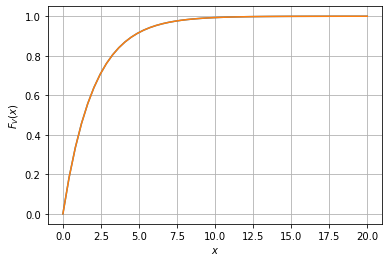
\includegraphics[width=\columnwidth]{6.1.1 cdf.png}
\caption{CDF of $V$}
\label{fig:probman_trans_cdf_V}
\end{figure}
The CDF of V is plotted in \ref{fig:probman_trans_cdf_V} using the code below.
\begin{lstlisting}
https://github.com/AmulyaTallamraju/AI1103/blob/main/probman/codes/6.1.1_CDF.py
\end{lstlisting}
\begin{figure}[!ht]
\centering
\includegraphics[width=\columnwidth]{6.1.1 PDf.png}
\caption{PDf of $V$}
\label{fig:probman_trans_PDf_V}
\end{figure}
The PDf of V is plotted in \ref{fig:probman_trans_PDf_V} using the code below.
\begin{lstlisting}
https://github.com/AmulyaTallamraju/AI1103/blob/main/probman/codes/6.1.1_PDf.py
\end{lstlisting}


%\solution The following code generates the simulated CDF in Fig. \ref{fig:probman_trans_cdf_V}
% %
% \begin{figure}[!ht]
% \centering
% \includegraphics[width=\columnwidth]{figs/trans/cdf_V.png}
% \caption{CDF of $V$}
% \label{fig:probman_trans_cdf_V}
% \end{figure}
% %
% and the PDf in Fig. \ref{fig:probman_trans_PDf_V}
% %
% \begin{figure}[!ht]
% \centering
% \includegraphics[width=\columnwidth]{figs/trans/PDf_V.png}
% \caption{PDf of $V$}
% \label{fig:probman_trans_PDf_V}
% \end{figure}
%

\item
If
%
\begin{equation}
F_{V}(x) = 
\begin{cases}
1 - e^{-\alpha x} & x \geq 0 \\
0 & x < 0,
\end{cases}
\label{eq:probman_F_V_alpha}
\end{equation}
%
find $\alpha$.

\solution
For the value $\alpha=0.5$, the theory matches the simulation.
\begin{figure}[!ht]
\centering
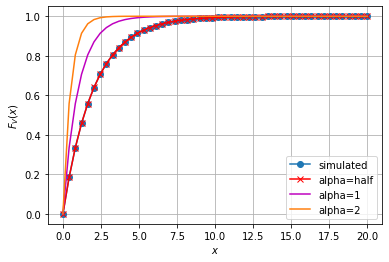
\includegraphics[width=\columnwidth]{6.1.2.png}
\caption{CDF of $V$}
\label{fig:probman_F_V_alpha}
\end{figure}
The CDF of V is plotted in \ref{fig:probman_F_V_alpha} using the code below.
\begin{lstlisting}
https://github.com/AmulyaTallamraju/AI1103/blob/main/probman/codes/6.1.2.py
\end{lstlisting}
%
\item
\label{ch3_raleigh_sim}
Plot the CDF and PDf of
%
\begin{equation}
A = \sqrt{V}
\end{equation}
%
\begin{figure}[!ht]
\centering
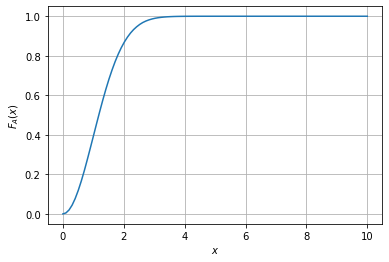
\includegraphics[width=\columnwidth]{6.1.3 cdf.png}
\caption{CDF of $A$}
\label{fig:probman_trans_cdf_A}
\end{figure}
The CDF of A is plotted in \ref{fig:probman_trans_cdf_A} using the code below.
\begin{lstlisting}
https://github.com/AmulyaTallamraju/AI1103/blob/main/probman/codes/6.1.3_CDF.py
\end{lstlisting}
\begin{figure}[!ht]
\centering
\includegraphics[width=\columnwidth]{6.1.3 PDf.png}
\caption{PDf of $V$}
\label{fig:probman_trans_PDf_A}
\end{figure}
The PDf of V is plotted in \ref{fig:probman_trans_PDf_V} using the code below.
\begin{lstlisting}
https://github.com/AmulyaTallamraju/AI1103/blob/main/probman/codes/6.1.3_PDf.py
\end{lstlisting}
%
\item
Find an expression for $F_{A}(x)$ using the definition. Plot this expression and compare with the result of problem \ref{ch3_raleigh_sim}. 
\\
\solution 

% Given,
% \begin{align}
% A = \sqrt{V}
% \end{align}

\begin{align} 
F_A(x) &= \pr{A \le x} = \pr{\sqrt{V} \le x}
\\
&= \pr{V \le x^2} = F_V\brak{x^2}
\end{align}
%
From \eqref{eq:probman_F_V_alpha}, 
\begin{align} 
F_V\brak{x^2} = 
\begin{cases}
1 - e^{-\alpha x^2} & x \geq 0 \\
0 & x < 0,
\end{cases}
\end{align}
%
Substituting 

\begin{align}
\alpha = \frac{1}{2}
\end{align}

%
\begin{align} 
F_V\brak{x^2} = 
\begin{cases}
1 - e^{- \frac{x^2}{2}} & x \geq 0 \\
0 & x < 0,
\end{cases}
\end{align}
\begin{figure}[!ht]
\centering
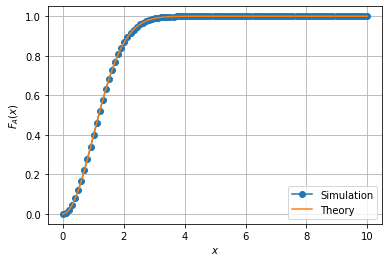
\includegraphics[width=\columnwidth]{6.1.4.png}
\caption{CDF of $A$}
\label{fig:probman_trans_cdf_A}
\end{figure}
The CDF of A is plotted in \ref{fig:probman_trans_cdf_A} using the code below.
\begin{lstlisting}
https://github.com/AmulyaTallamraju/AI1103/blob/main/probman/codes/6.1.4.py
\end{lstlisting}
%
\item
Find an expression for $p_{A}(x)$.
\\
\solution
The PDf is obtained as
\begin{align}
f_V\brak{x^2} &= \frac{d}{dx}F_V\brak{x^2}
\\
&=
\begin{cases}
x e^{- \frac{x^2}{2}} & x \geq 0 \\
0 & x < 0,
\end{cases}
\end{align}
The PDf of A is plotted in \ref{fig:probman_trans_pdf_A} using the code below.
\begin{lstlisting}
https://github.com/AmulyaTallamraju/AI1103/blob/main/probman/codes/6.1.5.py
\end{lstlisting}
\begin{figure}[!ht]
\centering
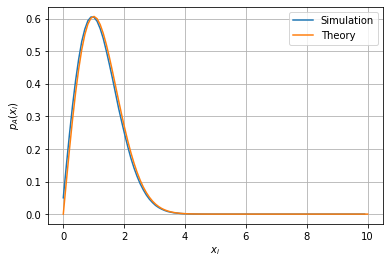
\includegraphics[width=\columnwidth]{6.1.5.png}
\caption{PDf of $A$}
\label{fig:probman_trans_pdf_A}
\end{figure}


%
\end{enumerate}



\end{document}
